% Chapter 15 of Volume III, "Chains at every level". Sources: misc/reviews/nick-volume3/vol3/ch8_chains.tex 7-40, 42-116, 118-140, 142-177, 179-237, 239-323, 325-399, 401-432, 434-463, 465-502, 504-518, 520-566 (condensed); reports U07 (ch8 part: M2 to M8 and minors) and V3D referee_chains.md; verification W5 V11. 17 Nov 2026.
\label{h:ch:chains}

\ifdefined\conjecture\else\theoremstyle{sc}\newtheorem{conjecture}[theorem]{Conjecture}\theoremstyle{scr}\fi
\ifdefined\computation\else\theoremstyle{sc}\newtheorem{computation}[theorem]{Computation}\theoremstyle{scr}\fi

The birth and death chain of Chapter~\ref{b:ch:chain}, the Krein string of the zeros of Section~\ref{bk:sec:string}, turns the Riemann Hypothesis into the positivity of one sequence of rates computed at the centre of the critical strip. This chapter, from an unrefereed note of Polson (November 2026), places that chain at the bottom of a family indexed by a level $\alpha>\frac12$. Write $\mathcal L$ for a completed $L$ function with real coefficients and $\mathcal L(s)=\mathcal L(1-s)$, so $\mathcal L=\xi$ for $\zeta$, and let $c_j$ be the rates of Chapter~\ref{b:ch:chain}, the rates of the S fraction of $G'/G$ with $G(u)=\xi(\frac12+\sqrt u)/\xi(\frac12)$. For each $\alpha$ the chain at level $\alpha$ is the S fraction of the odd to even quotient of $\mathcal L(\alpha+s)$.
Floating point computations are called computed, at the precision stated; agreement of two precisions is not a certificate, and nothing here is certified in ball arithmetic. The family proves nothing new about the zeros of $\zeta$. It shows where an arithmetic property must enter: the rungs at $\alpha\ge1$ are arithmetic theorems, and the Davenport and Heilbronn function, which has no Euler product, fails there in the computed cases (under regularity and for $\alpha$ outside a countable set, by Theorem~\ref{h:thm:crit}(ii)).

\section{The chain at level $\alpha$}

Let $K$ be an even kernel with $\mathcal L(\frac12+z)=\int_{\mathbb R}K(y)e^{zy}\,dy$. For $\xi$, $K$ is Riemann's $\Phi$. For the Davenport and Heilbronn function it is $e^{3y/2}\vartheta(e^{2y})$ with $\vartheta(x)=\sum na_ne^{-\pi n^2x/5}$. For $\alpha>\frac12$ put
\[
F_\alpha(s)=\frac{\mathcal L(\alpha+s)}{\mathcal L(\alpha)}=\sum_{n\ge0}f_n(\alpha)s^n,\qquad f_n(\alpha)=\frac{1}{\mathcal L(\alpha)}\int_{\mathbb R}K(y)e^{(\alpha-\frac12)y}\frac{y^n}{n!}\,dy,
\]
and split into even and odd parts,
\[
F_\alpha(s)=h_\alpha(s^2)+s\,g_\alpha(s^2),\qquad \varphi_\alpha(w)=\frac{g_\alpha(w)}{h_\alpha(w)}=\sum_{n\ge0}(-1)^nm_n(\alpha)w^n .
\]
The chain at level $\alpha$ is the Stieltjes continued fraction
\[
\varphi_\alpha(w)=\cfrac{m_0}{1+\cfrac{a_1(\alpha)w}{1+\cfrac{a_2(\alpha)w}{1+\cdots}}},
\]
computed from the moments $m_n(\alpha)$ by the same elimination as for the birth and death chain. We call it regular when all Hankel determinants of the $m_n$ are nonzero, so that every $a_j$ is defined.

\begin{lemma}[Phase]\label{h:lem:phase}
Let $\theta(t)=\arg F_\alpha(it)$, continuous with $\theta(0)=0$, on a line with no zero. Then
\[
\theta'(t)=\re\frac{\mathcal L'}{\mathcal L}(\alpha+it)=\sum_\rho\frac{\alpha-\beta}{(\alpha-\beta)^2+(t-\gamma)^2}=\pi\,u_\alpha(t),
\]
the Thorin density of Section~\ref{mi:sec:density}, for the real, functionally symmetric entire functions of order one with the canonical product convergence used there. If every $\beta<\alpha$, $\theta$ is strictly increasing.
\end{lemma}

This is Section~\ref{mi:sec:density} and the argument of Theorem~\ref{cx:thm:positivity}, so we do not repeat the proof.

\begin{theorem}[Criterion]\label{h:thm:crit}
Let $\alpha>\frac12$.
\begin{enumerate}
\item If every zero $\rho=\beta+i\gamma$ of $\mathcal L$ has $\beta<\alpha$, then $\varphi_\alpha$ is a Stieltjes function and $m_0>0$. If moreover $\theta$ is unbounded, as it is for $\xi$ and for the Davenport and Heilbronn function, then the chain is regular and every $a_j(\alpha)>0$.
\item Conversely, suppose $m_0>0$ and the chain is regular with every $a_j(\alpha)>0$. Then $F_\alpha$ has no zero $s_0$ with $\re s_0>0$ and $F_\alpha(-s_0)\ne0$. In particular $\mathcal L$ has no zero with $\beta>\alpha$, unless there is a second zero $\beta'+i\gamma$ at the same ordinate with $\beta+\beta'=2\alpha$.
\end{enumerate}
\end{theorem}

\begin{proof}
(i) Write $r$ for the zeros of $F_\alpha$, which are $\rho-\alpha$, so $\re r<0$. For $\re s<0$ the factor $|r-s|/|r+\bar s|$ is less than one, since $r$ and $s$ lie on the same side of the imaginary axis. The product over all zeros equals $|F_\alpha(s)/F_\alpha(-s)|$, the exponential factors cancelling by the identity above and $|F_\alpha(-\bar s)|=|F_\alpha(-s)|$ since $F_\alpha$ is real. Hence $S(s)=F_\alpha(s)/F_\alpha(-s)$ has $|S|<1$ for $\re s<0$. Put $s=iz$. Then
\[
\psi(z)=i\,\frac{1-S(iz)}{1+S(iz)}=\frac{z\,g_\alpha(-z^2)}{h_\alpha(-z^2)}=z\,\varphi_\alpha(-z^2)
\]
has positive imaginary part for $\im z>0$, and is odd and meromorphic. By the Nevanlinna representation of such functions \cite[Chapter~VII]{Levin64}, its poles are real and simple, and
\[
\psi(z)=\eta z+\sum_k c_k\Bigl(\frac{1}{t_k-z}-\frac1{t_k}\Bigr),\qquad \eta\ge0,\ c_k>0,
\]
with $\pm t_k$ the poles (the zeros of $h_\alpha(-z^2)$ not cancelled by $g_\alpha$). By Lemma~\ref{h:lem:phase} the phase is strictly increasing, so $\tan\theta=g_\alpha/h_\alpha$ has no cancellation: the $t_k$ are the points with $\theta(t_k)=(k-\frac12)\pi$, and $c_k=1/\theta'(t_k)$. Pairing $\pm t_k$ and dividing by $z$ gives
\[
\varphi_\alpha(w)=\eta+\sum_k\frac{W_k}{w+t_k^2},\qquad W_k=\frac{2}{\theta'(t_k)}=\frac{2}{\pi u_\alpha(t_k)}>0 ,
\]
a Stieltjes function, the transform $\int d\nu(x)/(1+xw)$ of the positive measure $\nu=\eta\delta_0+\sum_k(W_k/t_k^2)\delta_{t_k^{-2}}$ on $[0,t_1^{-2}]$. So $m_0=\nu(\mathbb R)>0$. If $\theta$ is unbounded there are infinitely many atoms, all Hankel determinants are positive, and Stieltjes' theorem \cite{Stieltjes94} gives a regular chain with $a_j>0$.

(ii) A positive regular chain gives positive Hankel determinants of both forms, hence a positive measure $\nu$ with moments $m_n$. Since $\varphi_\alpha$ is analytic at $0$, $m_n\le CR^n$, so $\nu$ lives on $[0,R]$ and $\varphi_\alpha(w)=\int d\nu(x)/(1+xw)$. For $\re s>0$ and $x>0$, $s/(1+xs^2)=x^{-1}\,1/(s+x^{-1}/s)$ has positive real part, and so has $s\cdot1$. Hence $\re\,s\varphi_\alpha(s^2)>0$ and $1+s\varphi_\alpha(s^2)\ne0$. Let $F_\alpha(s_0)=0$ with $\re s_0>0$. If $h_\alpha(s_0^2)\ne0$ then $F_\alpha=h_\alpha(1+s\varphi_\alpha)$ does not vanish at $s_0$. So $h_\alpha(s_0^2)=0$, hence $s_0g_\alpha(s_0^2)=0$, hence $g_\alpha(s_0^2)=0$ and $F_\alpha(-s_0)=h_\alpha-s_0g_\alpha=0$. A zero $\rho=\beta+i\gamma$ with $\beta>\alpha$ gives $s_0=\rho-\alpha$ with $F_\alpha(-s_0)=0$ exactly when $\mathcal L$ vanishes at $2\alpha-\rho$, equivalently at its conjugate $(2\alpha-\beta)+i\gamma$.
\end{proof}

\begin{remark}\label{h:rem:proviso}
For polynomials, (i) and (ii) are the Routh and Hurwitz criterion in Stieltjes form. The proviso in (ii) is needed. A zero $s_0$ with $F_\alpha(s_0)=F_\alpha(-s_0)=0$ is a common zero of $h_\alpha$ and $g_\alpha$, invisible to $\varphi_\alpha$, and a function of the class can have such a zero to the right of the line with every rate positive. An example: $\Lambda(v)=R(v-\frac12)\bigl[\sinh(v-\frac12)/(v-\frac12)\bigr]^{10}$, with $R$ the even polynomial of degree eight whose zeros have real parts $\frac18,\frac38,\frac58,\frac78$ and ordinates $\pm1$, at $\alpha=\frac34$. The zeros at real parts $\frac78$ and $\frac58$ sum to $2\alpha$, and exact rational arithmetic gives $m_0=\frac{10112}{6497}$ and positive first rates $a_1=\frac{706624}{513263}$, $a_2=\frac{307200}{872239}$, $a_3=\frac{5056}{11041}$ (computed). % UNVERIFIED: values from the V3D referee report, Sec. 1; the normalisation of the rates there is the one of this chapter but was not rechecked here Zeros on $\re s=\alpha$ are one source of common zeros, not the only one. For $\zeta$ a violation needs three zeros at one ordinate, a coincidence that is not excluded.
\end{remark}

\section{The limit $\alpha\to\frac12$ is the birth and death chain}

\begin{theorem}[Limit]\label{h:thm:limit}
Let $G(u)=\mathcal L(\frac12+\sqrt u)/\mathcal L(\frac12)$. As $\delta=\alpha-\frac12\downarrow0$,
\[
\varphi_\alpha(w)=2\delta\,\frac{G'(w)}{G(w)}+O(\delta^2),\qquad a_j(\alpha)\to c_j
\]
for every $j$ for which the chain of $G'/G$ is regular, where $c_j$ are its rates.
\end{theorem}

\begin{proof}
$h_\alpha(s^2)=\frac12(F_\alpha(s)+F_\alpha(-s))=G(s^2)+O(\delta)$. For the odd part, the evenness of $\mathcal L(\frac12+s)$ gives $\mathcal L(\frac12+\delta+s)-\mathcal L(\frac12+\delta-s)=\mathcal L(\frac12+s+\delta)-\mathcal L(\frac12+s-\delta)=2\delta\mathcal L'(\frac12+s)+O(\delta^3)$, and $\mathcal L'(\frac12+s)=\mathcal L(\frac12)\,2s\,G'(s^2)$. Hence $g_\alpha(w)=2\delta G'(w)+O(\delta^2)$. Dividing gives $\varphi_\alpha$. Multiplying a function by a constant changes only $m_0$ in its S fraction, so the rates $a_j$, $j\ge1$, converge to those of $G'/G$, each being a rational function of finitely many moments.
\end{proof}

\begin{computation}\label{h:comp:limit}
For $\xi$ at $\alpha=\frac12+10^{-7}$, $300$ digits, the first $79$ coefficients $a_j(\alpha)$ agree with the rates $c_j$ of the birth and death chain to twelve significant digits, for example $a_{40}=9.70024290826\cdot10^{-5}$ on both sides. % UNVERIFIED: the draft numbers were reproduced by the referee at 800 digits (relative difference at most 4.3e-15), not by an independent chain computation of the coordinator
\end{computation}

So the family is continuous down to the centre, and the birth and death chain of Chapter~\ref{b:ch:chain} is its bottom rung. For $G$ the quotient $G'/G=\sum_\gamma1/(u+\gamma^2)$, over the positive ordinates with multiplicity, is a Stieltjes function exactly when every zero of $G$ is real and negative, because a zero of $G$ is a pole of $G'/G$ with positive integer residue and cannot cancel. So positivity of the birth and death rates is equivalent to RH, with no proviso.

\section{The Jacobi matrix as a function of the base point: a Lax pair and a line of fixed points}\label{lx:sec:lax}

This section, from a note of Polson and Sokolov (November 2026), moves the expansion point of $F$ along the positive axis instead of along the abscissa. Let $z_\rho=-(\rho-\frac12)^2/2$, one for each pair $\{\rho,1-\rho\}$, so that under RH $z=\gamma^2/2$ with $\gamma>0$. For $u_0>0$ put $x_\rho=1/(u_0+z_\rho)$ and $\mu_{u_0}=\sum_\rho x_\rho\delta_{x_\rho}$. Its moments are $m_n(u_0)=\sum_\rho x_\rho^{n+1}=(-1)^nF^{(n)}(u_0)/n!$ with $F(u)=\sum_\rho1/(u+z_\rho)=2(G'/G)(2u)$, so $\mu_0$ is the measure of Chapter~\ref{b:ch:chain} with its atoms doubled. When the Hankel determinants of the $m_n(u_0)$ are nonzero (positive under RH), the orthonormal polynomials $p=(p_0,p_1,\dots)^{\top}$ satisfy $tp=Jp$ with $J=J(u_0)$ symmetric tridiagonal, diagonal $a_k$ and off diagonal $b_k$, and by the criterion at the end of the previous section, applied at $u_0$, RH holds if and only if every Hankel determinant is positive, that is every $b_k$ is defined and $b_k^2>0$, at one $u_0$ or at all. Since $dx_\rho/du_0=-x_\rho^2$, the flow is $\frac{d}{du_0}\int f\,d\mu=\int\dot f\,d\mu-\int t\,(tf)'\,d\mu$. In the scaled variables $\alpha_k=u_0a_k$, $\beta_k=u_0^2b_k^2$ and $\sigma=\log u_0$, Theorem~\ref{lx:thm:lax} becomes the autonomous lattice
\begin{gather*}
\frac{d\alpha_k}{d\sigma}=\alpha_k-\alpha_k^2-(2k+2)\beta_k+(2k-2)\beta_{k-1},\\
\frac{d\beta_k}{d\sigma}=2\beta_k\bigl[1-\alpha_k-\alpha_{k+1}+(k+\tfrac12)(\alpha_k-\alpha_{k+1})\bigr].
\end{gather*}
The Chebyshev point $C_1$ is $\alpha_k=\frac12$, $\beta_0=\frac18$, $\beta_k=\frac1{16}$ for $k\ge1$, the Jacobi coefficients of the arcsine law on $[0,1]$.

\begin{theorem}[Lax form]\label{lx:thm:lax}
Let $\Lambda=\mathrm{diag}(k+\frac12)$ and let $B=J_-\Lambda-\Lambda J_+$, where $J_\mp$ are the strictly lower and upper parts of $J$, so that $B$ is skew and tridiagonal with $B_{k+1,k}=(k+\frac12)b_k$. Then $\dot J=-J^2+[B,J]$.
\end{theorem}

\begin{proof}
Write $tp'=Mp$ with $M$ lower triangular, $M_{kk}=k$, and $\dot p=Ap$ with $A$ lower triangular. Differentiating $tp=Jp$ in $t$ and multiplying by $t$ gives $[J,M]=J$. Differentiating $\int p_ip_j\,d\mu=\delta_{ij}$ in $u_0$ with the flow above gives $A+A^{\top}=JM+JM^{\top}$. Put $A=JM-\frac12J+B$. The transpose $M^{\top}J=JM^{\top}+J$ of $[J,M]=J$ turns the identity into $B+B^{\top}=0$. As $A$ is lower triangular, the strictly upper part of $B$ is minus that of $JM-\frac12J$, which lives on the first superdiagonal and equals $(k+1)b_k-\frac12b_k$. So $B$ is as stated. Finally $\dot J=[A,J]=J[M,J]+[B,J]=-J^2+[B,J]$.
\end{proof}

The diagonal of $-J^2+[B,J]$ is $-a_k^2-(2k+2)b_k^2+(2k-2)b_{k-1}^2$, the second off diagonals cancel, and the first off diagonal gives $\dot b_k=b_k[-(a_k+a_{k+1})+(k+\frac12)(a_k-a_{k+1})]$. The Lax form of the Toda lattice is due to Flaschka and Moser \cite{Flaschka74,Moser75}, and the orthonormal polynomial derivation follows Szeg\H o and Chihara \cite{Szego39,Chihara78}.

\begin{corollary}[Isospectral form]\label{lx:cor:iso}
For a measure with finitely many atoms, wherever $J$ is invertible, $L=J^{-1}-u_0$ satisfies $\dot L=[B,L]$, and the eigenvalues of $L$ are the atoms $z$.
\end{corollary}

\begin{proof}
$\frac{d}{du_0}J^{-1}=-J^{-1}\dot JJ^{-1}=I-J^{-1}[B,J]J^{-1}=I+[B,J^{-1}]$.
\end{proof}

This is not true of finite sections. The leading $N\times N$ block obeys $\dot J_N=-J_N^2+[B_N,J_N]-2Nb_{N-1}^2e_{N-1}e_{N-1}^{\top}$, and at the zeta moments the eigenvalues of $J_N^{-1}-u_0$, reciprocal Gauss nodes minus $u_0$, move with $u_0$, though under RH they stay above $z_1=\gamma_1^2/2$. For zeta under RH, $J$ is a bounded injective self adjoint operator with unbounded inverse, and $L$ is unitarily equivalent to multiplication by $z$ on $\ell^2$ of the atoms. That is a reweighting of a fixed spectrum built from the zeros, as in the generalised Toda flows of Moser and of Deift, Nanda and Tomei \cite{Moser75,DNT83}, except that the tridiagonal matrix is $J$ and not $L$. It gives no new equivalence with RH: positivity of the $b_k^2$ at one $u_0$ or at all is the criterion above.

\begin{theorem}[Line of fixed points]\label{lx:thm:line}
For $0<\theta<2$ let $C_\theta$ be the Jacobi coefficients of the probability weight proportional to $y^{-\theta/2}(1-y)^{\theta/2-1}$ on $[0,1]$. Each $C_\theta$ is a fixed point of the autonomous lattice, with $\alpha_k=\frac12+\frac{\theta-1}{2(2k-1)(2k+1)}$ and $\beta_0=\frac12(1-\frac\theta2)\frac\theta2$, and $C_1$ is the Chebyshev point. If a positive measure with atoms $z=r^2/2$ has a counting function $N$ regularly varying of index $\theta$, then its orbit converges to $C_\theta$ as $u_0\to\infty$.
\end{theorem}

\begin{proof}
With $r=\sqrt{2u_0}\,\varrho$ and $N(r)=cr^\theta$ the scaled moments are $\int y^{n+1}dN=\frac12c\theta(2u_0)^{\theta/2}B(n+1-\frac\theta2,\frac\theta2)$, the moments of $y^{-\theta/2}(1-y)^{\theta/2-1}dy$ up to a factor depending on $u_0$ only. Jacobi coefficients do not see that factor, so $\alpha_k,\beta_k$ are constant in $\sigma$. For regularly varying $N$ write $\int y^{n+1}dN=\int N(r)\,d\bigl(-(1+r^2/2u_0)^{-n-1}\bigr)$ and apply Karamata's theorem \cite{BGT87} with dominated convergence. The values $\alpha_0,\beta_0$ are the mean and variance of the Beta$(1-\frac\theta2,\frac\theta2)$ law.
\end{proof}

For zeta the smooth count, with density $\frac1{2\pi}\log\frac r{2\pi}\,dr$, is regularly varying of index $1$, and the same integrals give, exactly for the smooth density, with $\Lambda=\log(\sqrt{2u_0}/2\pi)$, $\alpha_0=\frac12(1-1/\Lambda)$ and $\beta_0=\frac18-\frac1{4\Lambda^2}$. (The local exponent $d\log N/d\log r=1+1/\log(r/2\pi e)$ would put $2\pi e$ in place of $2\pi$; it is the moment integral, not the local exponent, that gives $2\pi$.) So the effective exponent $\theta_{\mathrm{eff}}=2(1-\alpha_0)$ is $1+1/\Lambda$, which explains the slow $1/\log u_0$ approach to $C_1$. At $u_0=5\cdot10^4$ the true orbit gives $\theta_{\mathrm{eff}}=1.2517$ (computed) against $1.2552$ from the formula. In the direction of $\beta_0$ the orbit leaves the line at second order, since $\beta_0(C_\theta)=\frac18-\frac{(\theta-1)^2}8$ is half the displacement $\frac1{4\Lambda^2}$ of the orbit, so the motion is along the line only to first order.

\begin{remark}[Heuristic: the resolution scale]
The $N$ point Gauss rule of the arcsine law has first node at ordinate $\gamma\approx\pi\sqrt{2u_0}/4N$ when mapped to the atoms $y=1/(1+\gamma^2/2u_0)$. It cannot tell the first zero $\gamma_1=14.1347\ldots$ from the smooth density while $N\lesssim K(u_0):=\pi\sqrt{2u_0}/(4\gamma_1)$, which is $5.6$ at $u_0=5000$ and $17.6$ at $u_0=5\cdot10^4$. This is a heuristic and nothing is proved about $K$. The data do not locate it: at $u_0=5000$ the deviation $|\alpha_k-\frac12|$ grows steadily from $0.0018$ at $k=2$ to $0.010$ at $k=10$ (computed), with no visible change at $K=5.6$.
\end{remark}

The Davenport and Heilbronn function is expected to flow to the same fixed point in the far field (Theorem~\ref{lx:thm:line} does not apply, since its atoms are not all real), and its chain at the centre is already computed in Section~\ref{b:sec:dh}. Theorem~\ref{lx:thm:lax} holds for it wherever its Jacobi matrix exists, so a proof has to use a property that function lacks, the Euler product being the obvious candidate.

\section{The chain is a quadrature of the Thorin measure}

The proof of Theorem~\ref{h:thm:crit}(i) says more than positivity. It identifies the measure of the chain.

\begin{theorem}[Quadrature]\label{h:thm:quad}
Let $\alpha>\frac12$ and suppose every zero has $\beta<\alpha$. Let $N_\alpha(t)=\int_0^tu_\alpha$ be the accumulated Thorin mass on the line $\re s=\alpha$, and let $t_k$ solve $N_\alpha(t_k)=k-\frac12$. Then
\[
\varphi_\alpha(w)=\eta+\sum_{k\ge1}\frac{W_k}{w+t_k^2},\qquad W_k=\frac{2}{\pi\,u_\alpha(t_k)} .
\]
The chain at level $\alpha$ is the Jacobi matrix of the discrete measure with atoms $t_k^{-2}$ and masses $W_kt_k^{-2}$, together with the mass $\eta$ at $0$: the Thorin measure sampled at its half integer quantiles, each atom weighted by the local spacing, since $\pi u_\alpha(t_k)(t_{k+1}-t_k)\approx\pi$.
\end{theorem}

Under RH, and if the zeros are simple, the birth and death chain is the limit. As $\delta\downarrow0$, $u_\alpha$ tends to a sum of point masses at the ordinates $\gamma_k$ of the zeros on the line, $N_\alpha$ becomes a staircase, the half integer levels are crossed at the steps, so $t_k\to\gamma_k$, and the Cauchy kernel of height $1/(\pi\delta)$ gives $W_k\to2\delta$. Then $\varphi_\alpha(w)\to\sum_k2\delta/(w+\gamma_k^2)=2\delta\,G'(w)/G(w)$, which is Theorem~\ref{h:thm:limit} again.

\begin{computation}\label{h:comp:quad}
Compute $\theta(t)=\arg\mathcal L(\alpha+it)$ on a grid, unwrap it, find the nodes $t_k$ by Newton's method and the weights $2/\theta'(t_k)$ from the analytic derivative, for $t\le200$ ($\xi$) or $t\le130$ (Davenport and Heilbronn), and compare $m_n=\sum_kW_kt_k^{-2(n+1)}$ with the kernel moments. The entries are relative differences (computed). The two Davenport and Heilbronn columns lie outside the hypothesis of Theorem~\ref{h:thm:quad}: that function has zeros to the right of both levels (for example $0.8085+85.70i$ inside the window at $\alpha=0.75$, where $\theta$ decreases, Computation~\ref{h:comp:dip}). They compare the node sum with the moments and are not evidence for the theorem.
\begin{center}\small
\begin{tabular}{@{}lccc@{}}
\toprule
& $\xi$, $\alpha=0.75$ & DH, $\alpha=0.85$ & DH, $\alpha=0.75$\\
\midrule
nodes & $79$ & $75$ & $73$\\
$m_2$ & $2.4\cdot10^{-6}$ & $5.4\cdot10^{-8}$ & $1.4\cdot10^{-7}$\\
$m_4$ & $3.6\cdot10^{-11}$ & $6.9\cdot10^{-14}$ & $1.0\cdot10^{-12}$\\
$m_6$ & $<10^{-16}$ & $1.1\cdot10^{-15}$ & $<10^{-16}$\\
\bottomrule
\end{tabular}
\end{center}
% UNVERIFIED: not rerun by the referees (DH columns are outside the theorem, see the text)
\end{computation}

\section{How a zero to the right is seen: the phase budget}

\begin{proposition}[Phase budget]\label{h:prop:budget}
Over the whole line, a zero $\rho$ with $\beta>\alpha$ contributes a Cauchy kernel of mass $-\pi$ to $\theta'$, and a zero with $\beta<\alpha$ contributes $+\pi$. So a zero to the right of $\re s=\alpha$ and its partner $1-\bar\rho$ together contribute $0$, against $+2\pi$ for a pair to the left: each zero to the right lowers the total phase by $2\pi$ relative to the count of zeros.
\end{proposition}

This is Proposition~\ref{cx:prop:deficit}, with the integral of the Cauchy kernel $\pi\operatorname{sign}(\alpha-\beta)$. Over a finite window or over positive ordinates only the mass is a difference of arctangents, and the loss is exactly $2\pi$ only in the limit.

\begin{remark}[Heuristic]\label{h:rem:budget}
It is natural to say that two half integer levels are lost, that two zeros of $h_\alpha$ leave the negative real axis as a complex pair or return as nodes of negative weight, and that the chain then has negative rates, two in every computed case. We have no proof. The statement would follow from Theorem~\ref{h:thm:inertia}, which is conditional, and in the class of functions with common zeros of $h_\alpha$ and $g_\alpha$ it is false (Remark after Theorem~\ref{h:thm:crit}).\end{remark}

\begin{computation}\label{h:comp:dip}
For the Davenport and Heilbronn zero $0.8085+85.70i$, $\theta(t)/\pi$ on $83\le t\le89$ is increasing at $\alpha=0.85$ and crosses four half integer levels. Below $\beta$ it crosses two, and it decreases on a short interval around $85.7$ by $0.84$, $0.58$, $0.42$, $0.19$, $0.10$ (in units of $\pi$) at $\alpha=0.80$, $0.75$, $0.70$, $0.60$, $0.55$ (computed).
% the five drops were recomputed by the V3D referee (0.838894, 0.577908, 0.424443, 0.194781, 0.095605)
\end{computation}

The dip shrinks as $\alpha$ approaches $\frac12$. Positivity of $u_\alpha$ on one line is necessary for no zero to the right and not known to be sufficient (Proposition~\ref{cx:prop:deficit}, Remark~\ref{rem:ch2:oneline}); the next proposition gives the first order form of why.

\begin{proposition}[Dipole]\label{h:prop:dipole}
Let $\delta=\alpha-\frac12$ and let a pair of zeros $\frac12\pm b+i\gamma_0$ lie off the line, $0<\delta<b$. Their joint contribution to $\pi u_\alpha(\gamma_0+x)$ is
\[
\frac{b+\delta}{(b+\delta)^2+x^2}-\frac{b-\delta}{(b-\delta)^2+x^2}=2\delta\,\frac{x^2-b^2}{(x^2+b^2)^2}+O(\delta^3),
\]
a signed dipole of total mass zero and central depth $2\delta/(b^2-\delta^2)$, with leading value $2\delta/b^2$. The zeros on the line contribute $\delta\sum_\gamma(\gamma_0+x-\gamma)^{-2}+O(\delta^2)$ away from their ordinates, also of order $\delta$. Hence, to first order in $\delta$ and if no other zero is off the line, $u_\alpha(\gamma_0)\ge0$ as soon as $\sum_\gamma(\gamma_0-\gamma)^{-2}>2/b^2$, which holds once the local density of zeros is large compared with $1/b$.
\end{proposition}

So pointwise positivity of the Thorin measure is necessary for positivity of the chain but not sufficient: at large height and $\alpha$ near $\frac12$, an off line pair can leave $u_\alpha\ge0$ at its own ordinate. The chain still sees it, because the phase budget counts zeros and not signs (the forward direction of Theorem~\ref{h:thm:crit} holds, and in Computations~\ref{h:comp:dip} and~\ref{h:comp:dipolehigh} the sign of $u_\alpha$ also detects a zero close to the line $\re s=\alpha$ relative to the local spacing).

\begin{computation}\label{h:comp:dipolehigh}
Take smooth zeros $N(t)=\frac{t}{2\pi}\log\frac{t}{2\pi e}+\frac78=k-\frac12$ within $4000$ zeros of a height $\gamma_0$, a far field from the density, and replace the zero nearest $\gamma_0$ by the quartet $\frac12\pm b\pm i\gamma_0$. The minimum of $u_\alpha$ on $[\gamma_0-3,\gamma_0+3]$ is (computed):
\begin{center}\small
\begin{tabular}{@{}lccc@{}}
\toprule
$(b,\alpha)$ & $\gamma_0=10^6$ & $\gamma_0=10^8$ & $\gamma_0=10^{10}$\\
\midrule
spacing & $0.525$ & $0.379$ & $0.297$\\
$(0.45,0.51)$ & $+0.0066$ & $+0.048$ & $+0.090$\\
$(0.30,0.55)$ & $-0.175$ & $+0.071$ & $+0.265$\\
$(0.20,0.55)$ & $-0.660$ & $-0.382$ & $-0.184$\\
\bottomrule
\end{tabular}
\end{center}
At low height (the Davenport and Heilbronn zero at $85.7$, and planted pairs at $90$, $5000$, $15000$, $18000$) the density always dips. At large height a pair far from the line, with $b$ comparable to the spacing, leaves $u_\alpha>0$ in this window, while the Thorin mass in the window falls by one unit against the count of the original zeros, two against the count of the zeros of the new configuration. The far field is an approximation and the window is finite, so this is a numerical statement, not a bound outside the window. % UNVERIFIED: the referee reproduced the values approximately; not rerun here
\end{computation}

\section{The chain counts the zeros to the right}\label{h:sec:count}

Write the chain as a continued fraction in $1/s$:
\[
s\,\varphi_\alpha(s^2)=\cfrac{1}{e_1s^{-1}+\cfrac{1}{e_2s^{-1}+\cfrac{1}{e_3s^{-1}+\cdots}}},
\]
with $e_1=1/m_0$ and $e_je_{j+1}=1/a_j$. The sign of $e_{j+1}$ is the sign of $m_0a_1\cdots a_j$: a negative rate is a sign change in the sequence $e_1,e_2,\dots$, and the $e_j$ are, up to positive factors, the terms $\sigma_0,\sigma_0',\sigma_1,\sigma_1',\dots$ of Section~\ref{h:sec:inertia}. For polynomials the $e_j$ are the Routh quotients.

\begin{proposition}[Routh count for polynomials]\label{h:prop:routh}
Let $p(s)=h(s^2)+sg(s^2)$ be a real polynomial of degree $d$ with $p(0)=1$ and no zero on the imaginary axis, in the regular case. Then the number of negative terms among $e_1,\dots,e_d$ equals the number of zeros of $p$ in $\re s>0$.
\end{proposition}

\begin{proof}
Apply Routh's theorem \cite{Gantmacher59} to the reversed polynomial $s^dp(1/s)$, whose zeros $1/s_\rho$ lie in the same half planes: the number of zeros in the right half plane is the number of sign changes in the first column $r_0,\dots,r_d$ of its Routh array, and the quotients $r_{j-1}/r_j$ are the $e_j$ up to positive factors.
\end{proof}

\begin{computation}\label{h:comp:routh}
For $60$ random real polynomials of degree $4$ to $14$ with zeros in both half planes, the number of negative $e_j$ equals the number of zeros in $\re s>0$ in all $60$. The number of negative rates $a_j$ does not: it agrees in only $11$ of the $60$ (computed). % UNVERIFIED: not rerun
\end{computation}

So the invariant that counts zeros is the number of negative terms $e_j$, not the number of negative rates. The two agree when each zero to the right produces an isolated adjacent pair of negative terms, as in every chain computed here, where the zeros to the right are far apart in level. It is a property of these spectra, not a general theorem.

\begin{conjecture}[Local count]\label{h:conj:count}
For $\alpha>\frac12$ and $J$ large, the number of negative terms $e_j$, $j\le J$, equals twice the number of zeros of $\mathcal L$ with $\beta>\alpha$ and $0<\gamma<H_J$, where $H_J$ is the turning height of level $J$, up to boundary effects at the last few levels. The negative terms attached to one zero are adjacent and separated from those of other zeros by positive terms, so that the number of negative rates is the same.
\end{conjecture}

Every computation in this chapter agrees with it: for the Davenport and Heilbronn function, $2$ negative terms and $2$ negative rates at $\alpha=0.80$, $0.75$, $0.66$ (one zero to the right below height $150$), $4$ at $\alpha=0.64$ and $0.55$ (two zeros), none at $\alpha\ge0.82$. For $\xi$ there is none at any rung computed.

\begin{theorem}[Upper bound]\label{h:thm:upper}
Suppose $\mathcal L$ has exactly $k$ zeros with $\beta>\alpha$, $\gamma>0$, no real zero with $\beta>\alpha$, none with $\beta=\alpha$, and that the chain at level $\alpha$ and the chains of the partial products below are regular. Then the sequence $e_1,e_2,\dots$ of the chain has at most $2k$ negative terms, and the chain has at most $4k$ negative rates.
\end{theorem}

\begin{proof}
Let $p_N(s)=\prod_{|\gamma|<T_N}(1-s/s_\rho)$ be the symmetric partial products. Their Taylor coefficients converge to those of $F_\alpha$: the power sums $\sum s_\rho^{-n}$, $n\ge2$, converge absolutely, and for $n=1$ the imaginary parts cancel in conjugate pairs while $\sum\re(1/s_\rho)=-\mathcal L'/\mathcal L(\alpha)$ converges absolutely (Lemma~\ref{h:lem:phase}). Each $e_j$ is a rational function of finitely many Taylor coefficients, so $e_j(p_N)\to e_j$ for fixed $j$. By Proposition~\ref{h:prop:routh}, $p_N$ has at most $2k$ negative terms in all. If the limit sequence had $2k+1$ negative terms among its first $J$, so would $p_N$ for large $N$, a contradiction. Each negative term accounts for at most two sign changes.
\end{proof}

\begin{corollary}[Eventual positivity]\label{h:cor:eventual}
If only finitely many zeros lie to the right of $\re s=\alpha$, none of them real and none with $\beta=\alpha$, and the regularity hypotheses of Theorem~\ref{h:thm:upper} hold, then all but finitely many rates $a_j(\alpha)$ are positive. At the bottom rung: if $\mathcal L$ has $k_0$ zeros with $\beta>\frac12$, $\gamma>0$, and no real zero with $\beta>\frac12$, and the chain of $G'/G$ and the chains at the levels $\alpha\in(\frac12,\frac12+\varepsilon)$ outside a countable set and their partial products are regular, then at most $4k_0$ of the birth and death rates $c_j$ are negative, so all but finitely many are positive.
\end{corollary}

\begin{proof}
The first statement is Theorem~\ref{h:thm:upper}. For the second, if $4k_0+1$ of the $c_j$ were negative, then, since $a_j(\alpha)\to c_j$ (Theorem~\ref{h:thm:limit}) and a strictly negative limit persists, the same $4k_0+1$ rates would be negative at every $\alpha$ close enough to $\frac12$. But for $\alpha>\frac12$ at most $k_0$ zeros lie to the right, so Theorem~\ref{h:thm:upper} allows at most $4k_0$. The levels with a zero on $\re s=\alpha$ are countable and are avoided.
\end{proof}

This does not interchange the limits $j\to\infty$ and $\alpha\to\frac12$: it uses the bound that is uniform in $\alpha$. At the bottom rung the same bound follows from Theorem~\ref{thm:ch12:inertia}, as in Remark~\ref{b:rem:eventual}. The exact count of $2k$ negative terms needs the theory of Krein and Langer (next section), or a proof that the negative terms of $p_N$ do not escape to infinity as $N$ grows.

\begin{computation}[Planted quartets in the $\xi$ chain]\label{h:comp:plant}
Multiply $\xi(\alpha+s)$ by the quartic with zeros at $\frac12\pm b\pm i\gamma_0$, so that the true zeros of $\zeta$ are kept and one quartet off the line is added, and compute the chain from the kernel moments. Runs at $700$ and $880$ digits agree through $j=209$ (computed).
\begin{center}\small
\begin{tabular}{@{}llll@{}}
\toprule
$\alpha$ & planted $(b,\gamma_0)$ & to the right of $\alpha$ & negative rates\\
\midrule
$0.51$ & $(0.05,60)$ & one & $68$, $70$\\
$0.51$ & $(0.2,60)$ & one & $66$, $68$\\
$0.51$ & $(0.4,60)$ & one & $63$, $65$\\
$0.51$ & $(0.2,40)$ & one & $37$, $39$\\
$0.51$ & $(0.2,85)$ & one & $95$, $97$\\
$0.51$ & $(0.2,110)$ & one & $133$, $135$\\
$0.75$ & $(0.2,60)$ & none & none\\
$0.75$ & $(0.4,60)$ & one & $64$, $66$\\
$0.51$ & $(0.2,50)$ and $(0.3,95)$ & two & $44$, $46$, $122$, $124$\\
$0.60$ & $(0.05,50)$ and $(0.3,95)$ & one & $123$, $125$\\
\bottomrule
\end{tabular}
\end{center}
% UNVERIFIED: the table was not rerun; only the smooth law levels below were recomputed (W5 V11)
\end{computation}

Within $j\le209$ the count is exact in all ten cases: two negative rates for each quartet with $\frac12+b>\alpha$, none for a quartet to the left, and the last row shows the chain selecting only the zero that is to the right of its own line. A zero only $0.05$ from the critical line is caught as cleanly as one at $0.4$. The level grows with the ordinate and falls slightly as $b$ grows ($68$, $66$, $63$). It sits about $12$ to $19$ levels above the level $\frac{\gamma_0}{2}\log\frac{\gamma_0}{4\pi}+\frac74$ of the smooth law ($24.9$, $83.0$, $121.1$ for $\gamma_0=40$, $85$, $110$, and $48.65$ for $\gamma_0=60$); we have not derived the shift.

\section{Toward a proof of the count: the inertia theorem}\label{h:sec:inertia}

The count can be reduced to the theory of generalised Schur and Nevanlinna functions of Krein and Langer. We give the reduction with proofs of the steps that are ours, and we state the two results taken from the literature as hypotheses.

Let $D_n=\det(m_{i+j})_{i,j<n}$ and $D'_n=\det(m_{i+j+1})_{i,j<n}$, with $D_0=D_0'=1$, and put $\sigma_n=D_{n+1}/D_n$, $\sigma'_n=D'_{n+1}/D'_n$.

\begin{lemma}[Rates and Hankel ratios]\label{h:lem:ratios}
In the regular case, $a_{2n+1}=\sigma'_n/\sigma_n$ and $a_{2n}=\sigma_n/\sigma'_{n-1}$. Hence $a_j<0$ exactly at the sign changes of the interleaved sequence $\sigma_0,\sigma'_0,\sigma_1,\sigma'_1,\dots$, and by Jacobi's rule the number of negative $\sigma_i$, $i<n$, is the number of negative squares $\nu_n$ of the Hankel form $(m_{i+j})_{i,j<n}$; likewise $\nu_n'$ for the shifted form and the $\sigma'_i$.
\end{lemma}

\begin{proof}
These are the classical determinant formulas for the coefficients of an S fraction \cite{Stieltjes94}, written as ratios, together with Jacobi's signature rule.
\end{proof}

Call a zero $s_0$ of $F_\alpha$ with $\re s_0>0$ unpaired if $F_\alpha(-s_0)\ne0$. By the proof of Theorem~\ref{h:thm:crit}(ii) only unpaired zeros are seen by $\varphi_\alpha$.

\begin{lemma}[Blaschke factorisation]\label{h:lem:blaschke}
Suppose $F_\alpha$ has exactly $\kappa$ unpaired zeros in $\re s>0$, counted with multiplicity, and none on the imaginary axis. Let $P$ be the real polynomial with these zeros and $E=F_\alpha/P$. Then for $\re s<0$
\[
S(s):=\frac{F_\alpha(s)}{F_\alpha(-s)}=\frac{S_E(s)}{\mathcal B(s)},\qquad S_E(s)=\frac{E(s)}{E(-s)},\qquad \mathcal B(s)=\frac{P(-s)}{P(s)},
\]
where $|S_E|<1$ and $\mathcal B$ is a Blaschke product of degree $\kappa$ for the left half plane with no zero in common with $S_E$.
\end{lemma}

\begin{proof}
By the product formula of Theorem~\ref{h:thm:crit}(i), $|F_\alpha(s)/F_\alpha(-\bar s)|=\prod_r|r-s|/|r+\bar s|$ over all zeros $r$. For a zero $r$ in $\re r>0$ the factor exceeds one when $\re s<0$, and it is compensated exactly by the factor of the zero $-r$ when $-r$ is also a zero (a paired zero), since the four factors of the quartet $r,-r,\bar r,-\bar r$ have product one. Dividing by the same product for $P$ leaves the product over the zeros of $E$, in which the paired zeros cancel in pairs and the remaining ones lie in $\re r<0$ with factor less than one. So $|S_E|<1$. The zeros of $\mathcal B$ are the reflections $-s_\rho$ of the unpaired zeros, which are not zeros of $F_\alpha$, hence not zeros of $E$.
\end{proof}

We state the two results from the literature as hypotheses, applied to $\varphi_\alpha$.
\begin{enumerate}
\item[(I1)] A quotient of a Schur function by a Blaschke product of degree $\kappa$ with no common zero is a generalised Schur function with exactly $\kappa$ negative squares \cite{KL77}, and the Cayley transform of such a function is a generalised Nevanlinna function with $\kappa$ negative squares.
\item[(I2)] For an odd generalised Nevanlinna function $\psi(t)=t\varphi(-t^2)$ with $\kappa$ negative squares, the index splits between $\varphi$ and $w\varphi$, so that the numbers of negative squares of the two Hankel forms add to $\kappa$.
\end{enumerate}
Here $S(it)=e^{2i\theta(t)}$ and the Cayley transform is $\psi=\tan\theta=g_\alpha/h_\alpha$ on the axis. We have not found a statement of (I2) in a source we could check.

\begin{theorem}[Inertia]\label{h:thm:inertia}
Assume (I1) and (I2) apply to $\varphi_\alpha$ and $m_0>0$. If $\mathcal L$ has exactly $k$ unpaired zeros with $\beta>\alpha$ and $\gamma>0$, no real unpaired zero with $\beta>\alpha$, none on $\re s=\alpha$, then in the regular case
\[
\nu+\nu'=2k,
\]
where $\nu$ and $\nu'$ are the numbers of negative terms among the $\sigma_n$ and the $\sigma'_n$. Consequently the chain at level $\alpha$ has at least $2$ and at most $4k$ negative rates when $k\ge1$, and exactly $2k$ if the negative terms occur in adjacent pairs $(\sigma_n,\sigma'_n)$ or $(\sigma'_n,\sigma_{n+1})$ separated by positive terms.
\end{theorem}

\begin{proof}
The unpaired zeros of $F_\alpha$ in $\re s>0$ are $s_\rho$ and $\bar s_\rho$ for the $k$ zeros in question, so $\kappa=2k$ by Lemma~\ref{h:lem:blaschke}, and the index is $\nu+\nu'$ by (I1) and (I2). By Lemma~\ref{h:lem:ratios} the negative rates are the sign changes of the interleaved sequence, which starts positive and, having finitely many negative terms, ends positive: the number of sign changes is even, at least $2$, and at most twice the number of negative terms. Adjacent pairs separated by positive terms give two sign changes for two negative terms.
\end{proof}

\begin{computation}\label{h:comp:inertia}
Reading the signs of $\sigma_n$ and $\sigma'_n$ from the computed rates: in all $21$ chains of this chapter (eight for Davenport and Heilbronn, three for $\xi$, ten with planted quartets) % TODO: the chapter's own computations show six $\xi$ chains in Computation~\ref{h:comp:xi}, so the count 21 needs the source
$\nu+\nu'=2k$ within the computed depth, with $k$ the number of zeros to the right that the depth resolves, with $\nu=\nu'=k$, and the negative terms always form adjacent pairs, for example terms $148,149$ and $218,219$ for Davenport and Heilbronn at $\alpha=0.55$ (computed). % UNVERIFIED: not rerun
\end{computation}

\begin{remark}[What remains for a full proof of the count]
Three things. First, (I1) and (I2) must be checked for $\varphi_\alpha$: the Krein and Langer factorisation is stated for the disc or half plane and needs $S_E$ to be a Schur function up to the boundary, and the splitting for odd functions must be matched to our sign conventions. Second, the adjacency of negative terms, $\nu=\nu'$ with isolated pairs, is observed in every case but not proved; it is what turns the bound $4k$ into the exact count $2k$. Third, locality, the level at which a pair appears, is not addressed by inertia.
\end{remark}

\section{The Euler product rungs made explicit}\label{h:sec:euler}

At $\alpha>1$ the positivity of the chain is a theorem (Theorem~\ref{h:thm:crit}(i) with $\zeta\ne0$ for $\re s>1$), and the arithmetic input of the Thorin density can be written down. For $s=\alpha+it$ the decomposition of Section~\ref{cf:sec:arith} (equation~\eqref{cf:eq:euler}) reads
\begin{multline*}
\pi u_\alpha(t)=\re\Bigl(\frac1s+\frac1{s-1}\Bigr)-\frac12\log\pi+\frac12\re\psi\Bigl(\frac s2\Bigr)+\re\frac{\zeta'}{\zeta}(s),\\ \Bigl|\re\frac{\zeta'}{\zeta}(s)\Bigr|\le\sum_n\frac{\Lambda(n)}{n^\alpha}=-\frac{\zeta'}{\zeta}(\alpha),
\end{multline*}
the bound coming from the Euler product. The Gamma part grows like $\frac12\log\frac{t}{2\pi}$, so $u_\alpha(t)>0$ for $t$ beyond a height of about $t_*(\alpha)=2\pi e^{-2\zeta'/\zeta(\alpha)}$. This $t_*$ is an indicative height, not a rigorous cutoff: it drops the term $\re(1/s+1/(s-1))$ and the error in $\psi$. Below $t_*$ a finite computation is needed.

\begin{computation}\label{h:comp:euler}
The values of $-\zeta'/\zeta(\alpha)$ and $t_*(\alpha)$ were recomputed at $40$ digits (computed); the entries for $t_*$ are rounded.
\begin{center}\small
\begin{tabular}{@{}lccc@{}}
\toprule
$\alpha$ & $-\zeta'/\zeta(\alpha)$ & $t_*(\alpha)$ & $\min u_\alpha$ on $[0,t_*]$, direct\\
\midrule
$2.0$ & $0.5700$ & $19.6$ & $+0.022$\\
$1.5$ & $1.5052$ & $127.5$ & $+0.015$\\
$1.3$ & $2.8081$ & $1726.9$ & $+0.012$\\
$1.2$ & $4.4583$ & $46843$ & not run\\
\bottomrule
\end{tabular}
\end{center}
% UNVERIFIED: the minima on [0,t_*] were not shown to be minima; the referee confirmed only the values u_alpha(0) = 0.0220, 0.0147, 0.0118
\end{computation}

Since $-\zeta'/\zeta(\alpha)\sim1/(\alpha-1)$, the finite range grows like a constant times $e^{2/(\alpha-1)}$ and the method of absolute bounds fails at $\alpha=1$. That is exactly where de la Vall\'ee Poussin's inequality $3+4\cos\theta+\cos2\theta\ge0$ replaces the absolute bound by a positivity argument that uses the Euler product three times at once (Section~\ref{cf:sec:arith}). Below $1$ no absolute bound exists at all, and every known argument for a zero free region is of the second kind.
\section{The ladder}

\begin{corollary}[Threshold]\label{h:cor:ladder}
Let $\beta^*=\sup\{\beta:\mathcal L(\beta+i\gamma)=0\}$ and assume the chains are regular. The chain at level $\alpha$ is positive for every $\alpha>\beta^*$. For $\frac12<\alpha<\beta^*$ it is not positive, except for the countable set of $\alpha$ at which every zero with $\beta>\alpha$ has a partner $\beta'+i\gamma$ with $\beta+\beta'=2\alpha$. Hence RH holds if and only if the chain is positive at every $\alpha>\frac12$, and if and only if the birth and death rates are positive.
\end{corollary}

\begin{proof}
The first assertion is Theorem~\ref{h:thm:crit}(i), and the second is (ii). For the last: if a zero has $\beta>\frac12$, choose $\alpha\in(\frac12,\beta)$ outside the countable set of midpoints $(\beta+\beta')/2$ of the real parts of zeros at that ordinate, and (ii) excludes positivity at $\alpha$. Conversely RH makes $\beta^*=\frac12$. Positivity of the birth and death rates is equivalent to RH by the remark after Computation~\ref{h:comp:limit}.
\end{proof}

For $\zeta$ the rungs that are known or claimed are these.
\begin{center}\small
\begin{tabular}{@{}p{0.17\textwidth}p{0.42\textwidth}p{0.32\textwidth}@{}}
\toprule
rung & reason & status\\
\midrule
$\alpha>1$ & Euler product: $\zeta(s)\ne0$ for $\re s>1$ & proved, classical\\
$\alpha=1$ & no zeros on $\re s=1$: $3+4\cos\theta+\cos2\theta\ge0$ & proved, Hadamard and de la Vall\'ee Poussin 1896\\
$\frac78<\alpha<1$ & zero free half plane & proved, \cite{OAI26a}; Section~\ref{qrh:sec:claims}\\
$\alpha\downarrow\frac12$ & RH & open\\
\bottomrule
\end{tabular}
\end{center}
The half plane $\frac78$ is the theorem of \cite{OAI26a}, discussed in Section~\ref{qrh:sec:claims}: positivity of the chain for every $\alpha>\frac78$ follows by Theorem~\ref{h:thm:crit}(i). The $\frac{11}{12}$ manuscript \cite{OAI26b} states a weaker exponent, which that theorem already covers. The rungs below $\frac78$ are open.

The rungs at and above $1$ are arithmetic. A Dirichlet series with periodic coefficients has no zeros in $\re s>1$ if and only if it is a Dirichlet polynomial with no zeros in $\re s>1$ times a Dirichlet $L$ function (Saias and Weingartner \cite{SaiasWeingartner09}). So among such series that also have the functional equation needed to define the chain, positivity of the chains at every $\alpha>1$ characterises the $L$ functions up to a polynomial factor. The Davenport and Heilbronn function has infinitely many zeros in $\re s>1$ \cite{DH36}, so its chain at $\alpha$ slightly above $1$ fails at some depth, for $\alpha$ outside a countable set and under regularity, by Theorem~\ref{h:thm:crit}(ii), while for $\zeta$ and every Dirichlet $L$ function of a real primitive character the chain is positive at all depths for $\alpha>1$.

\section{Calibration: the Davenport and Heilbronn phase diagram}

\begin{computation}\label{h:comp:phase}
For the Davenport and Heilbronn function, compute $a_j(\alpha)$ for $j\le249$ at $800$ and $1000$ digits. % UNVERIFIED: V3D reproduced the 800 digit run only; the 1000 digit agreement is the draft's claim
The two agree to $10^{-10}$ at every level and every $\alpha$ below, which is agreement of two floating point precisions and not a certificate. Negative rates appear at exactly these levels (computed).
\begin{center}\small
\begin{tabular}{@{}p{0.27\textwidth}p{0.28\textwidth}p{0.33\textwidth}@{}}
\toprule
$\alpha$ & negative rates & zeros with $\beta>\alpha$\\
\midrule
$1.00$, $0.90$, $0.82$ & none & none below height $150$\\
$0.80$ & $155$, $157$ & $0.8085+85.70i$\\
$0.75$ & $151$, $153$ & $0.8085+85.70i$\\
$0.66$ & $149$, $151$ & $0.8085+85.70i$\\
$0.64$ & $149$, $151$, $222$, $224$ & both, the second at $0.6508+114.16i$\\
$0.55$ & $148$, $150$, $218$, $220$ & both\\
\bottomrule
\end{tabular}
\end{center}
\end{computation}

\begin{figure}[ht]\centering
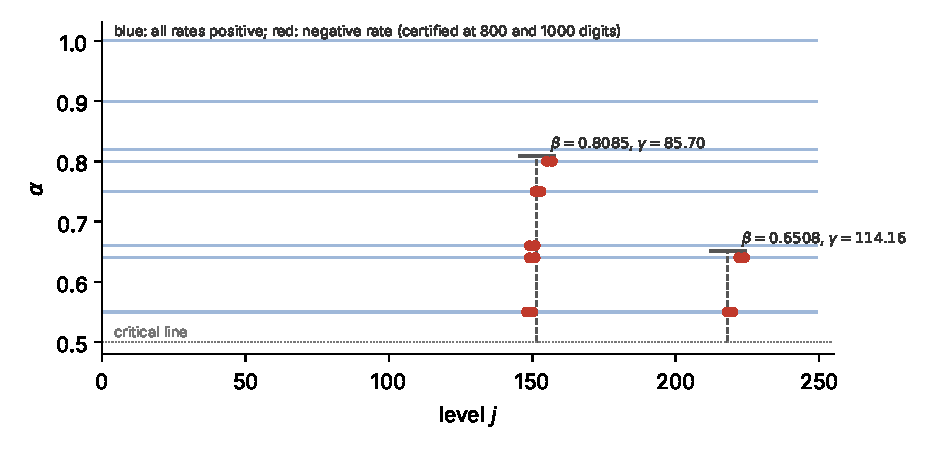
\includegraphics[width=\textwidth]{fig/v3/fig_phase.pdf}
\caption{Phase diagram of the Davenport and Heilbronn chains (computed). A rung at level $\alpha$ fails where a zero with $\beta>\alpha$ is reached; the dashed lines mark the levels $151.5$ and $218.1$ predicted by the Bohr and Sommerfeld law.}
\end{figure}

\begin{computation}\label{h:comp:scan}
Scan $\alpha$ across $\beta=0.808517$ at $700$ digits and record $r_j=a_j/\sqrt{a_{j-4}a_{j+4}}$ for $152\le j\le160$. At $\alpha=0.8090$ and $0.8086$, just above $\beta$, every $r_j$ lies between $0.92$ and $1.13$, the same range as at $\alpha=0.90$. At $\alpha=0.8084$, just below, the negative rates are $a_{161}$ and $a_{163}$ (computed). % UNVERIFIED: indices 161 and 163 from the V3D referee; the range 152 to 160 of r_j then does not contain them and should be rerun
\end{computation}

So positivity is not lost gradually: the rates give no warning that a zero is about to cross the line $\re s=\alpha$. Positive data do not measure the distance to the nearest bad zero.

\section{The ladder for $\zeta$}

\begin{computation}\label{h:comp:xi}
For $\xi$ at $\alpha=1$, $0.875$, $0.75$, $0.65$, $0.55$, $0.51$, the chains computed at $800$ and $1000$ digits agree through $j=249$ and every rate is positive. The smallest rate decreases slowly as $\alpha$ falls: $7.02\cdot10^{-6}$, $6.95\cdot10^{-6}$, $6.88\cdot10^{-6}$, $6.84\cdot10^{-6}$, $6.82\cdot10^{-6}$, $6.81\cdot10^{-6}$ (computed).
\end{computation}

\begin{computation}\label{h:comp:stab}
The $\xi$ rates are not monotone in $\alpha$: on $121$ of the $249$ levels, chiefly the death levels, $a_j$ rises between at least one pair of adjacent sampled values of $\alpha$ ($103$ rise between $\alpha=1$ and $\alpha=0.51$). They are stable: for every $j\le249$, $0.9028\le a_j(0.51)/a_j(1)\le1.0345$. Across the whole ladder from the Euler product rung to the edge of the critical line no rate of $\zeta$ moves by more than ten per cent, whereas the Davenport and Heilbronn rates change sign as $\alpha$ crosses $0.8085$ (computed).
\end{computation}

These are consistent with no zero of $\zeta$ with $\beta\ge0.51$ below the height these levels resolve, about $150$, which is far below what direct computation of zeros reaches. This is not a verification: Theorem~\ref{h:thm:crit} requires every $j$, and positivity of $249$ rates proves no exclusion height, since a real symmetric polynomial multiplier can insert an off line zero at any prescribed ordinate and leave the coefficients that determine the first $249$ rates unchanged.
\section{What this says about a path}

The ladder gives the problem a definite shape. A proof of RH by this route is a proof that the chain is positive at every rung, and the rungs that are known are known for arithmetic reasons: the Euler product above $1$, the inequality $3+4\cos\theta+\cos2\theta\ge0$ at $1$, and, if the claims stand, M\"obius amplification below. Each step down the ladder is a zero free half plane, and the bottom rung is RH. The chain does not make these steps easier. What it adds is the following.
\begin{enumerate}
\item The right object for the descent. Pointwise positivity of $U_\alpha$ can miss a zero when $\alpha$ is near the critical line (Proposition~\ref{h:prop:dipole}); the chain, a quadrature of $U_\alpha$ that keeps the phase budget, is not fooled in the cases computed.
\item A precise place for the arithmetic. The Davenport and Heilbronn function shares the Gamma factor, the functional equation and the Bohr and Sommerfeld law with the $L$ functions of conductor $5$, and its ladder is broken at the top. Any argument that would show positivity at a rung $\alpha<1$ must therefore use a property that the Davenport and Heilbronn function lacks, such as the Euler product used for the rungs at and above $1$.
\end{enumerate}
\begin{problem}
Remove the proviso of Theorem~\ref{h:thm:crit}(ii) for $\zeta$: show that $F_\alpha(s)$ and $F_\alpha(-s)$ have no common zero with $\re s>0$ (no two zeros of $\xi$ at one ordinate with real parts summing to $2\alpha$), or find a form of the criterion that does not need it.
\end{problem}

\begin{problem}
Give a proof of positivity of the rung $\alpha=1$ for $\zeta$ that runs through the rates, using the Euler product. Then try the same argument at $\alpha=\frac{11}{12}$.
\end{problem}

